In this section we describe in detail the results from our experimental evaluation, which consists of the generation of wordclouds, document duplicate detection and classification algorithm performance comparison.

\subsubsection{Wordcloud}
For each of the input set categories we generated the following wordclouds:

\begin{figure}[H]
\centering
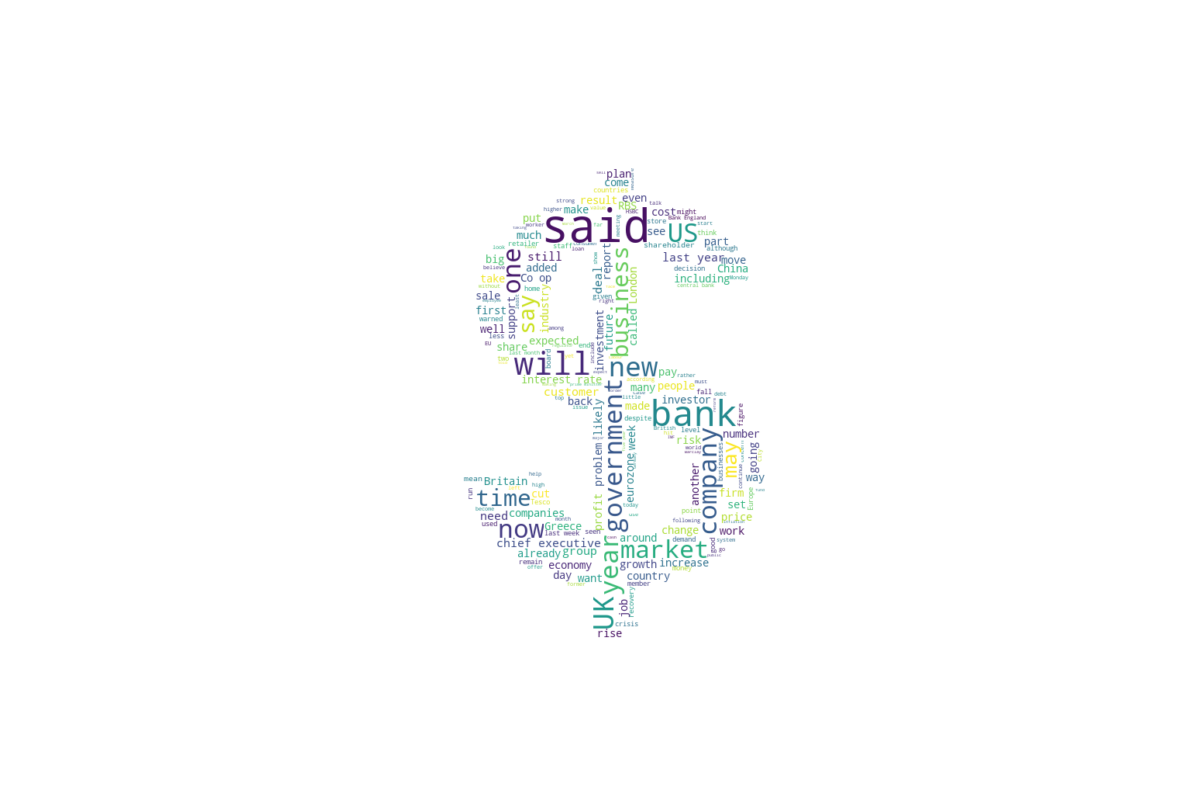
\includegraphics[scale=0.35]{images/Wordcloud_Business.png}
\caption{Business}
\end{figure}

\begin{figure}[H]
\centering
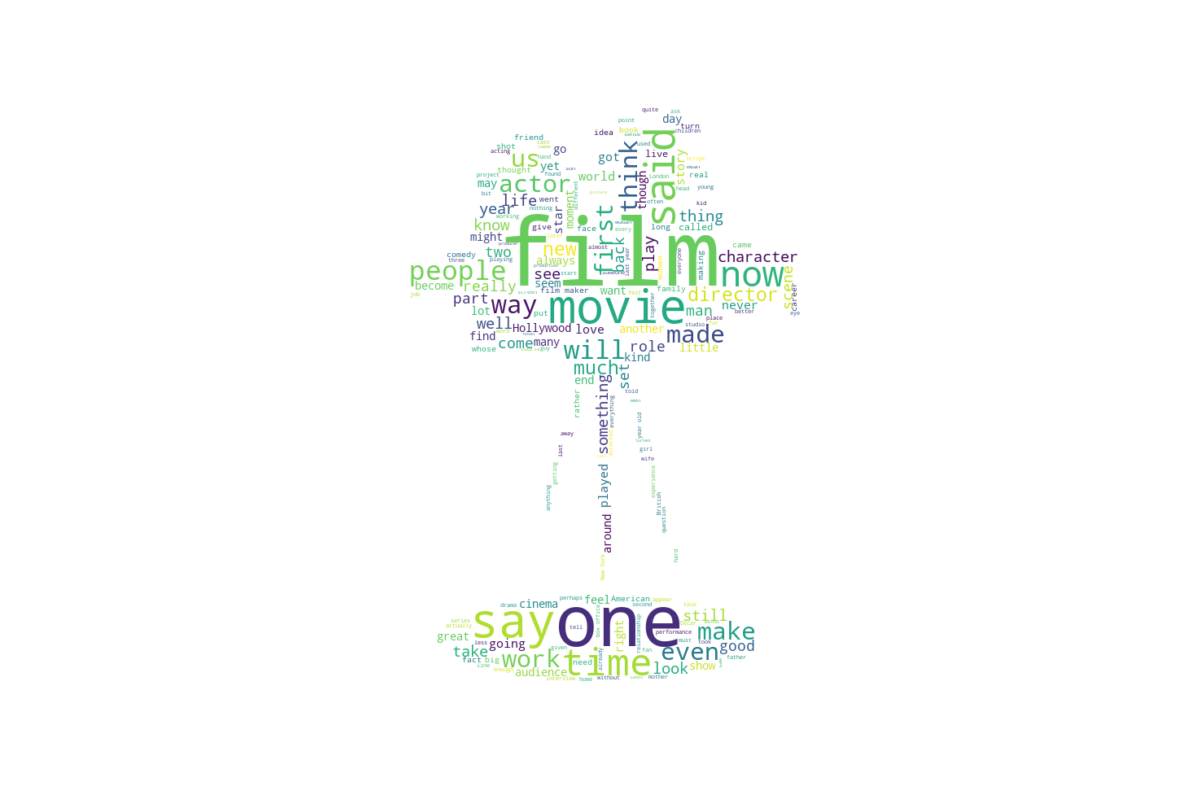
\includegraphics[scale=0.35]{images/Wordcloud_Film.png}
\caption{Film}
\end{figure}

\begin{figure}[H]
\centering
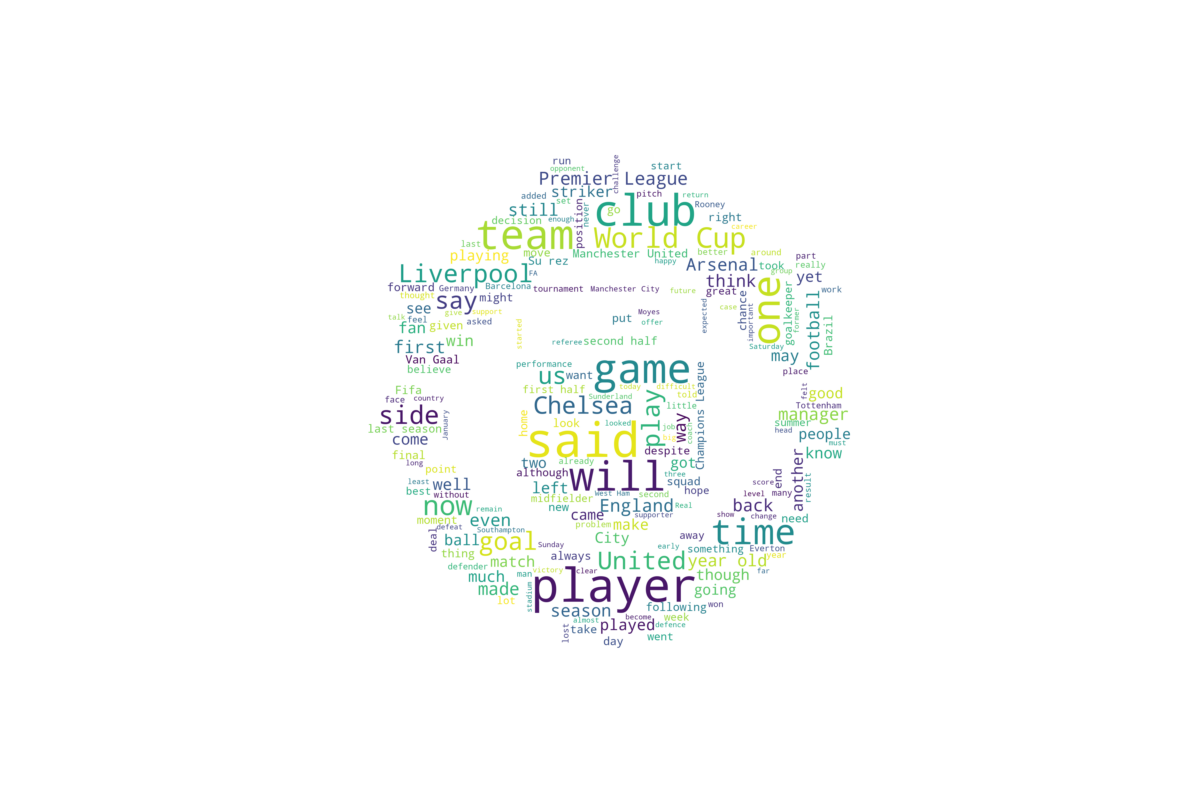
\includegraphics[scale=0.35]{images/Wordcloud_Football.png}
\caption{Football}
\end{figure}

\begin{figure}[H]
\centering
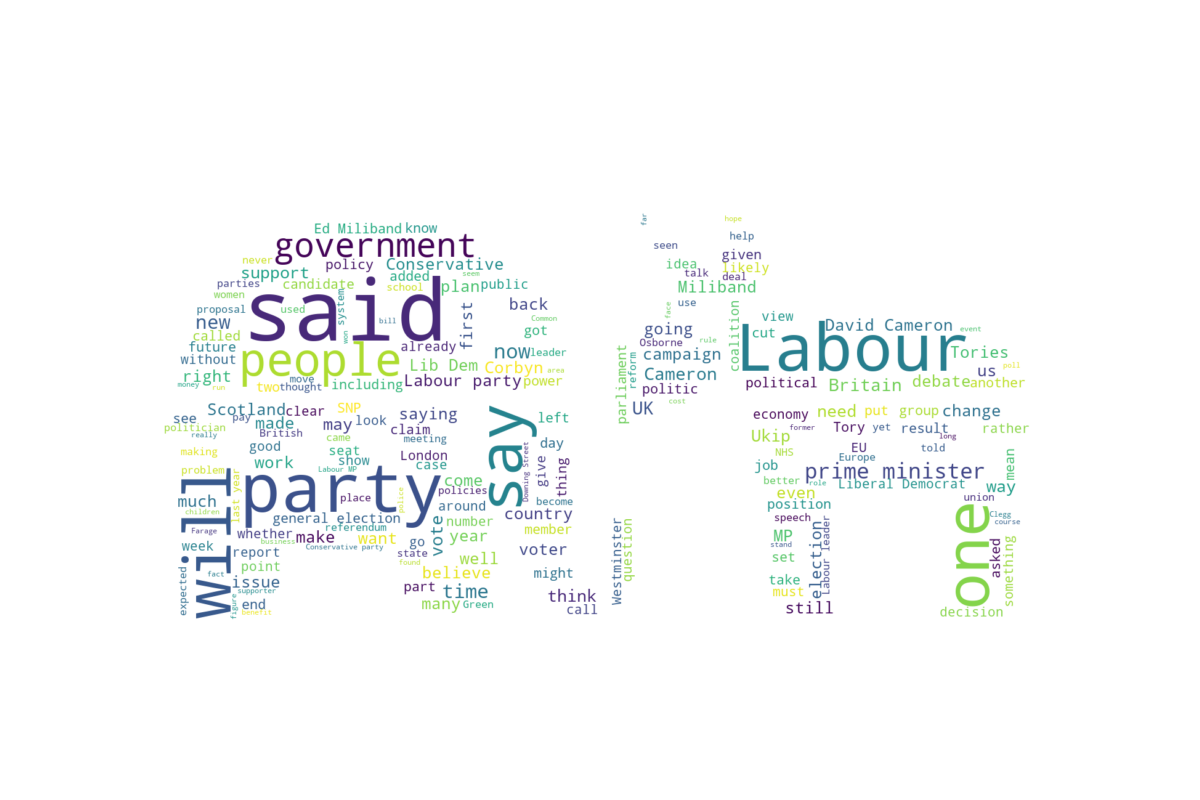
\includegraphics[scale=0.35]{images/Wordcloud_Politics.png}
\caption{Politics}
\end{figure}

\begin{figure}[H]
\centering
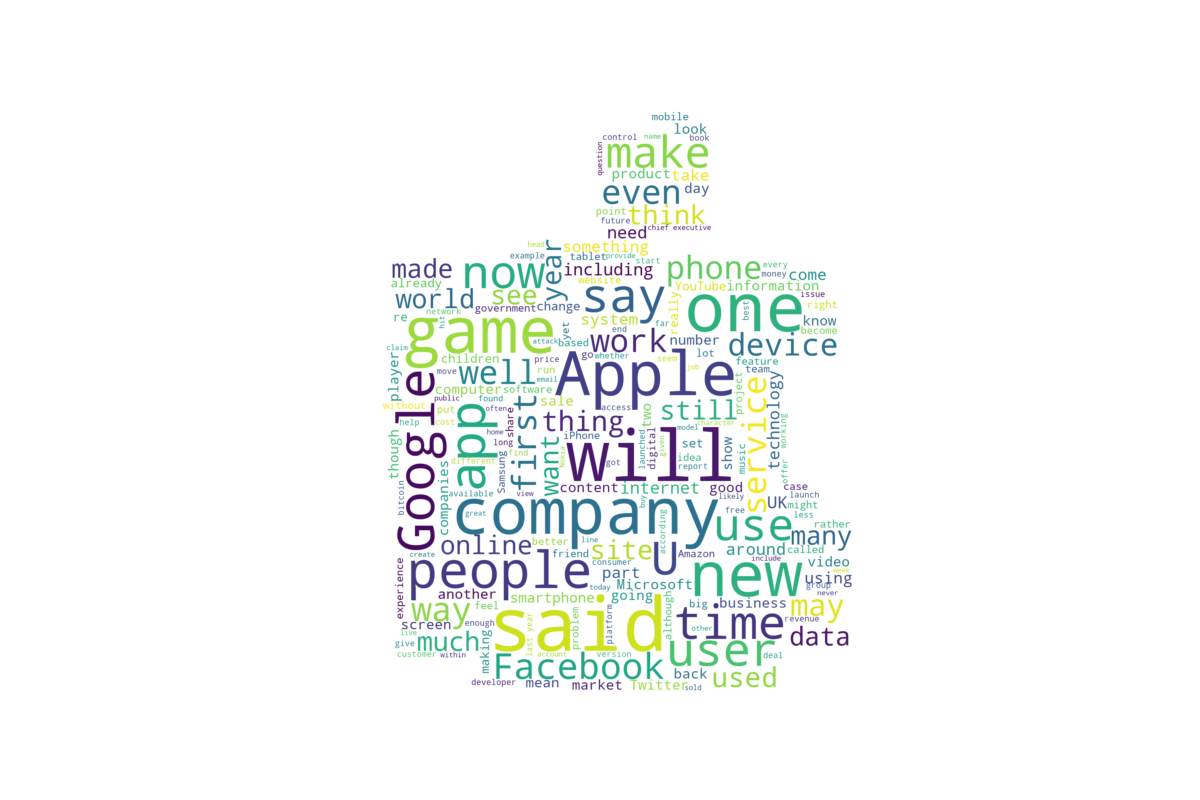
\includegraphics[scale=0.35]{images/Wordcloud_Technology.png}
\caption{Technology}
\end{figure}
\newpage
\subsubsection{Duplicates Detection}
As requested, the given source code accepts an input parameter $\theta$ as the similarity threshold. To export the results, we used $\theta = 0.7$ and based on this threshold, an output file (duplicatePairs.csv) is generated including all the document pairs with cosine similarity $>= 0.7$. Below is a small sample of the output file: \newline

\begin{tabular}{ |M{3cm}|M{3cm}|M{3cm}|  }
    \hline
    \rowcolor{lightgray!60}
    \multicolumn{3}{|c|}{duplicatePairs.csv} \\
    \hline 
    \rowcolor{lightgray!40}
    Document\_ID1& Document\_ID2 & Similarity \\
    \hline
    10802 & 10213 & 0.7104 \\
    10802 & 13991 & 0.7073 \\
    6727 & 1015 & 0.7134 \\
    ... & ... & ... \\
    7811 & 11213 & 0.7150 \\
    14607 & 11213 & 0.7661 \\
    \hline
\end{tabular}

\subsubsection{Classification Algorithms}
Below you can find the evaluation metric table which holds the performance of each classification algorithm implemented:

\begin{table}[H]
    \hspace{-50pt}
    \begin{tabular}{|>{\columncolor{lightgray!40}}l|l|l|l|l|l|l|l|l|l|}
        \hline
        \rowcolor{lightgray!40}
        Measure &  SVM(BoW) &  RF(BoW)  & SVM(SVD) & RF(SVD) & SVM(W2V) & RF(W2V)  & NN\\ \hline
        Accuracy & 0.935 & 0.927 & 0.931 & 0.929 & 0.935 & 0.889 & 0.964 \\ \hline
        Precision & 0.932 & 0.925 & 0.928 & 0.927 & 0.930 & 0.885 & 0.962 \\ \hline
        Recall & 0.929 & 0.916 & 0.925 & 0.920 & 0.929 & 0.878 & 0.961 \\ \hline
        F-Measure & 0.930 & 0.920 & 0.926 & 0.923 & 0.929 & 0.881 & 0.962 \\ \hline
        AUC & 0.956 & 0.949 & 0.954 & 0.951 & 0.956 & 0.925 & 0.976 \\ \hline
    \end{tabular}
    \caption{EvaluationMetric\_10fold.csv}
\end{table}
\noindent
Testing the performance of the MLP, using the token vectors from \textit{HashingVectorizer} we managed to achieve a performance increase over the methods used in subsection 3.3 as shown above, in the evaluation metric table (EvaluationMetric\_10fold.csv). The performance of this architecture was consistently better as there were multiple experiments with different seeds and inputs. With our custom architecture (Neural Network) we generated an output file (testSet\_categories.csv) which holds all the predicted categories for each document of the test set. The format of the output file is shown in the sample below:\\
\begin{table}[H]
\centering
\begin{tabular}{ |M{5cm}|M{5cm}|  }
    \hline
    \rowcolor{lightgray!60}
    \multicolumn{2}{|c|}{testSet\_categories.csv} \\
    \hline 
    \rowcolor{lightgray!40}
    Test\_Document\_ID & Predicted\_Category \\
    \hline
    2 & Politics \\
    10 & Technology \\
    25 & Technology \\
    ... & ... \\
    15332 & Football \\
    15333 & Football \\
    \hline
\end{tabular}
\end{table}

